\section{Introduction}
\vspace{-0.4em}
Ever since AlexNet \cite{krizhevsky2017imagenet} popularized deep learning in computer vision, the field has thrived under the reign of massive models with an ever increasing number of parameters. 
% Alarge number of 
Many
vision problems once considered difficult or impossible are now benchmark tasks: classification with tens of thousands of classes \cite{deng2009imagenet,zhou2017scene,gemmeke2017audio}, 
% accurate object detection \cite{ren2015faster,tian2019fcos,li2022exploring}, 
fast instance segmentation \cite{he2017mask,bolya2019yolact}, realistic image generation \cite{karras2018style,ho2020denoising,rombach2022high}, and more.

% There are a plethora of existing and carefully tuned models out there for many tasks. 
There are an abundance of independent, carefully tuned models out there for many tasks.
% While they often share the same core architectural backbone (e.g., ResNet-50, \citet{he2015deep}), they suffer from a potentially debilitating issue: they can only perform the task they were trained on. 
However, if we want to expand an existing model's capabilities, we run into many potential issues. If we try training the model on an additional task, we face catastrophic forgetting \cite{kirkpatrick2017overcoming,li2017learning,de2021continual}. If we evaluate the same model on different data without adaptation, we often find it doesn't generalize to out of domain samples \cite{blanchard2011generalizing,muandet2013domain,wang2022generalizing}. We can try so called ``intervention'' strategies \cite{wang2022generalizing,de2021continual} to mitigate these effects, but these often require further training which can be expensive~\cite{dosovitskiy2020image,zhai2022scaling,dehghani2023scalingvit22b}. 
Instead, it would be nice if we could expand a model's capacity to solve new tasks by simply ``zipping'' it with other models trained on those tasks \textit{without additional training}.
% Instead, it would be nice if we could simply ``zip'' these models together so that any \textcolor{red}{similar or} redundant features between them only need to be computed once, \textit{without} any additional training.



% \begin{figure}[b]
% \centering

% \begin{minipage}{0.48\linewidth}{
%     % \centering
%     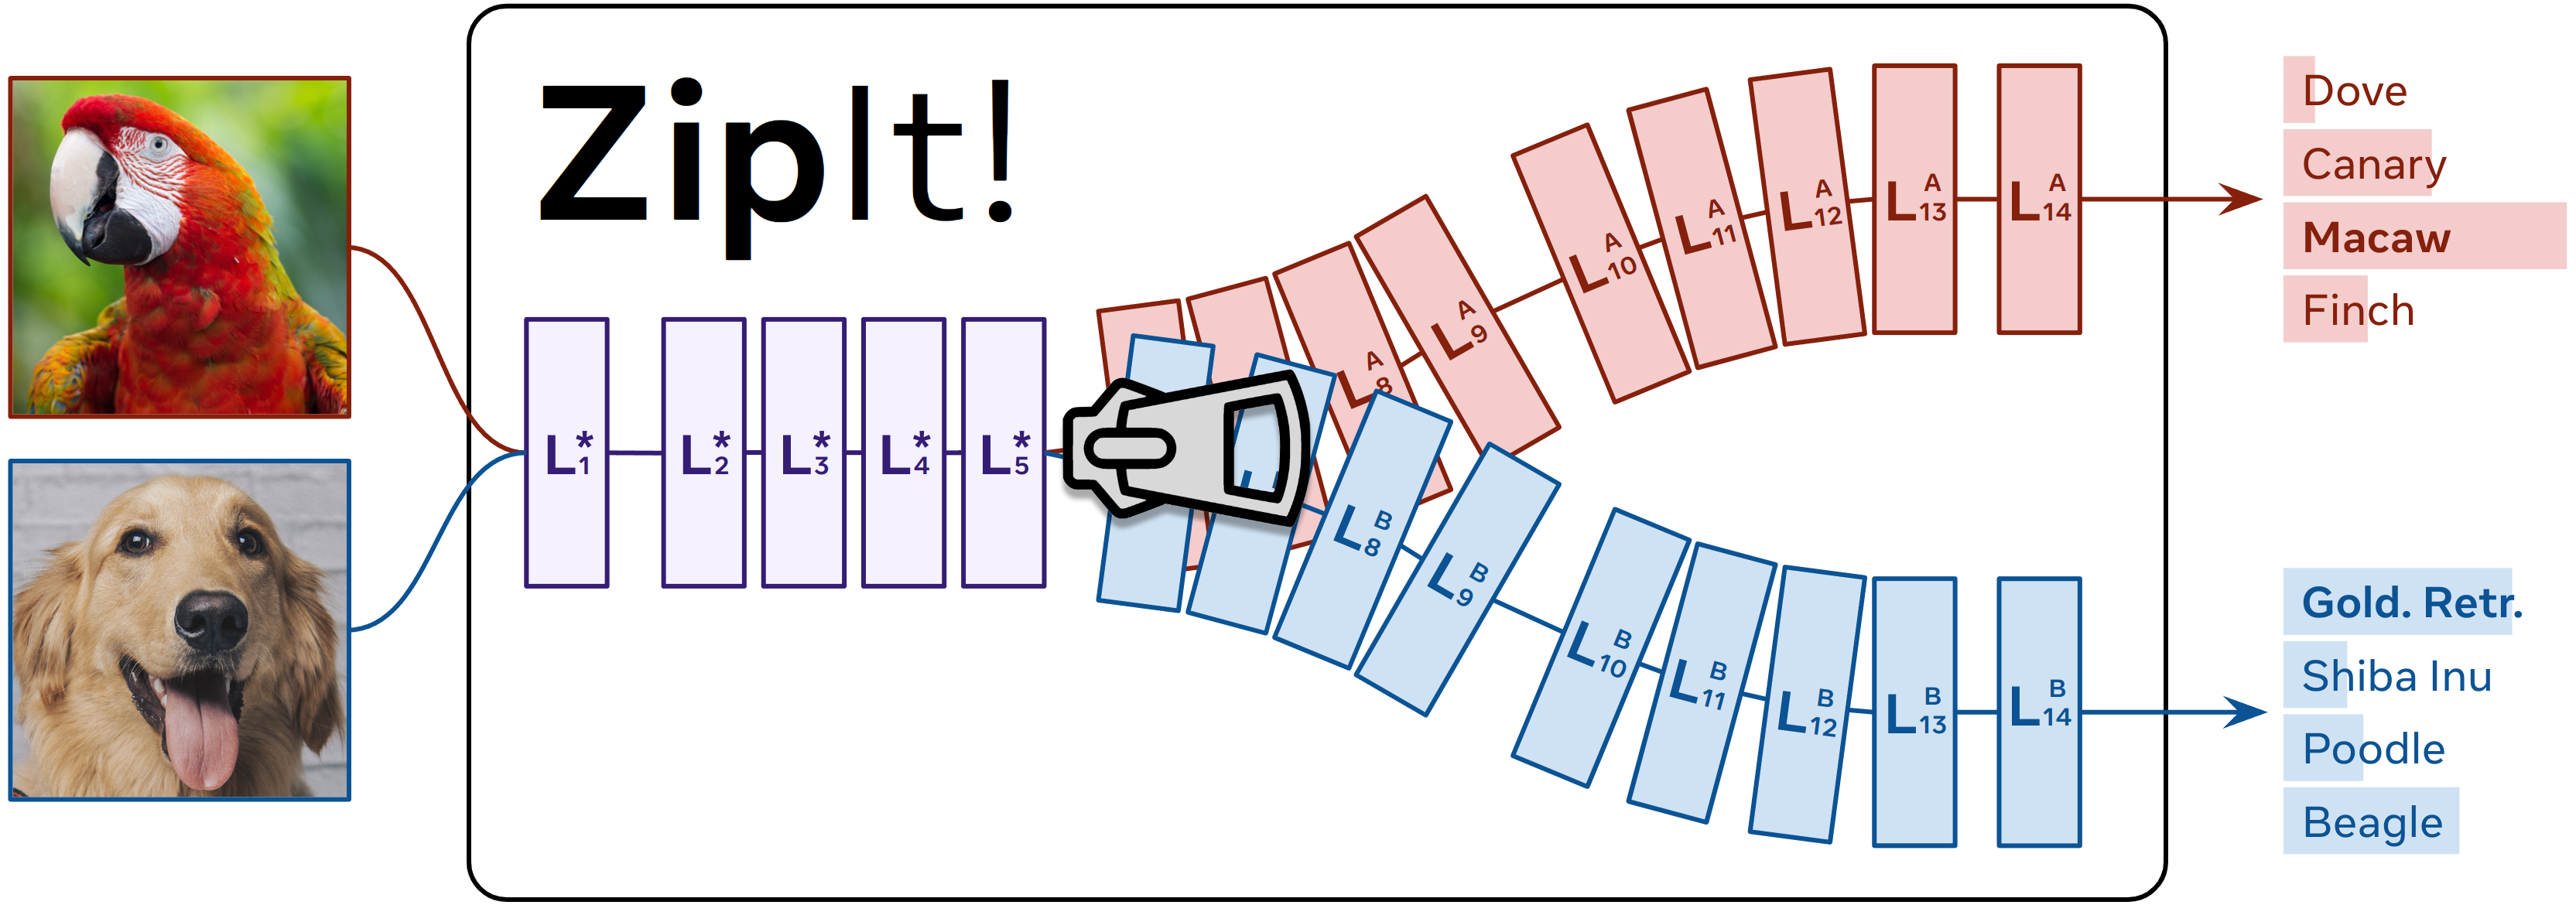
\includegraphics[width=\linewidth]{figures/imgs/concept.png}
%     \caption{{\bf \name{}} merges models trained on completely separate tasks \textit{without any additional training} by identifying their shared features.
%     Depending on the architecture and task, \name{} can nearly match their ensemble performance.
%     }
%     \label{fig:concept}
% }\end{minipage}
% \hspace{1em}
% \begin{minipage}{0.48\linewidth}{
%     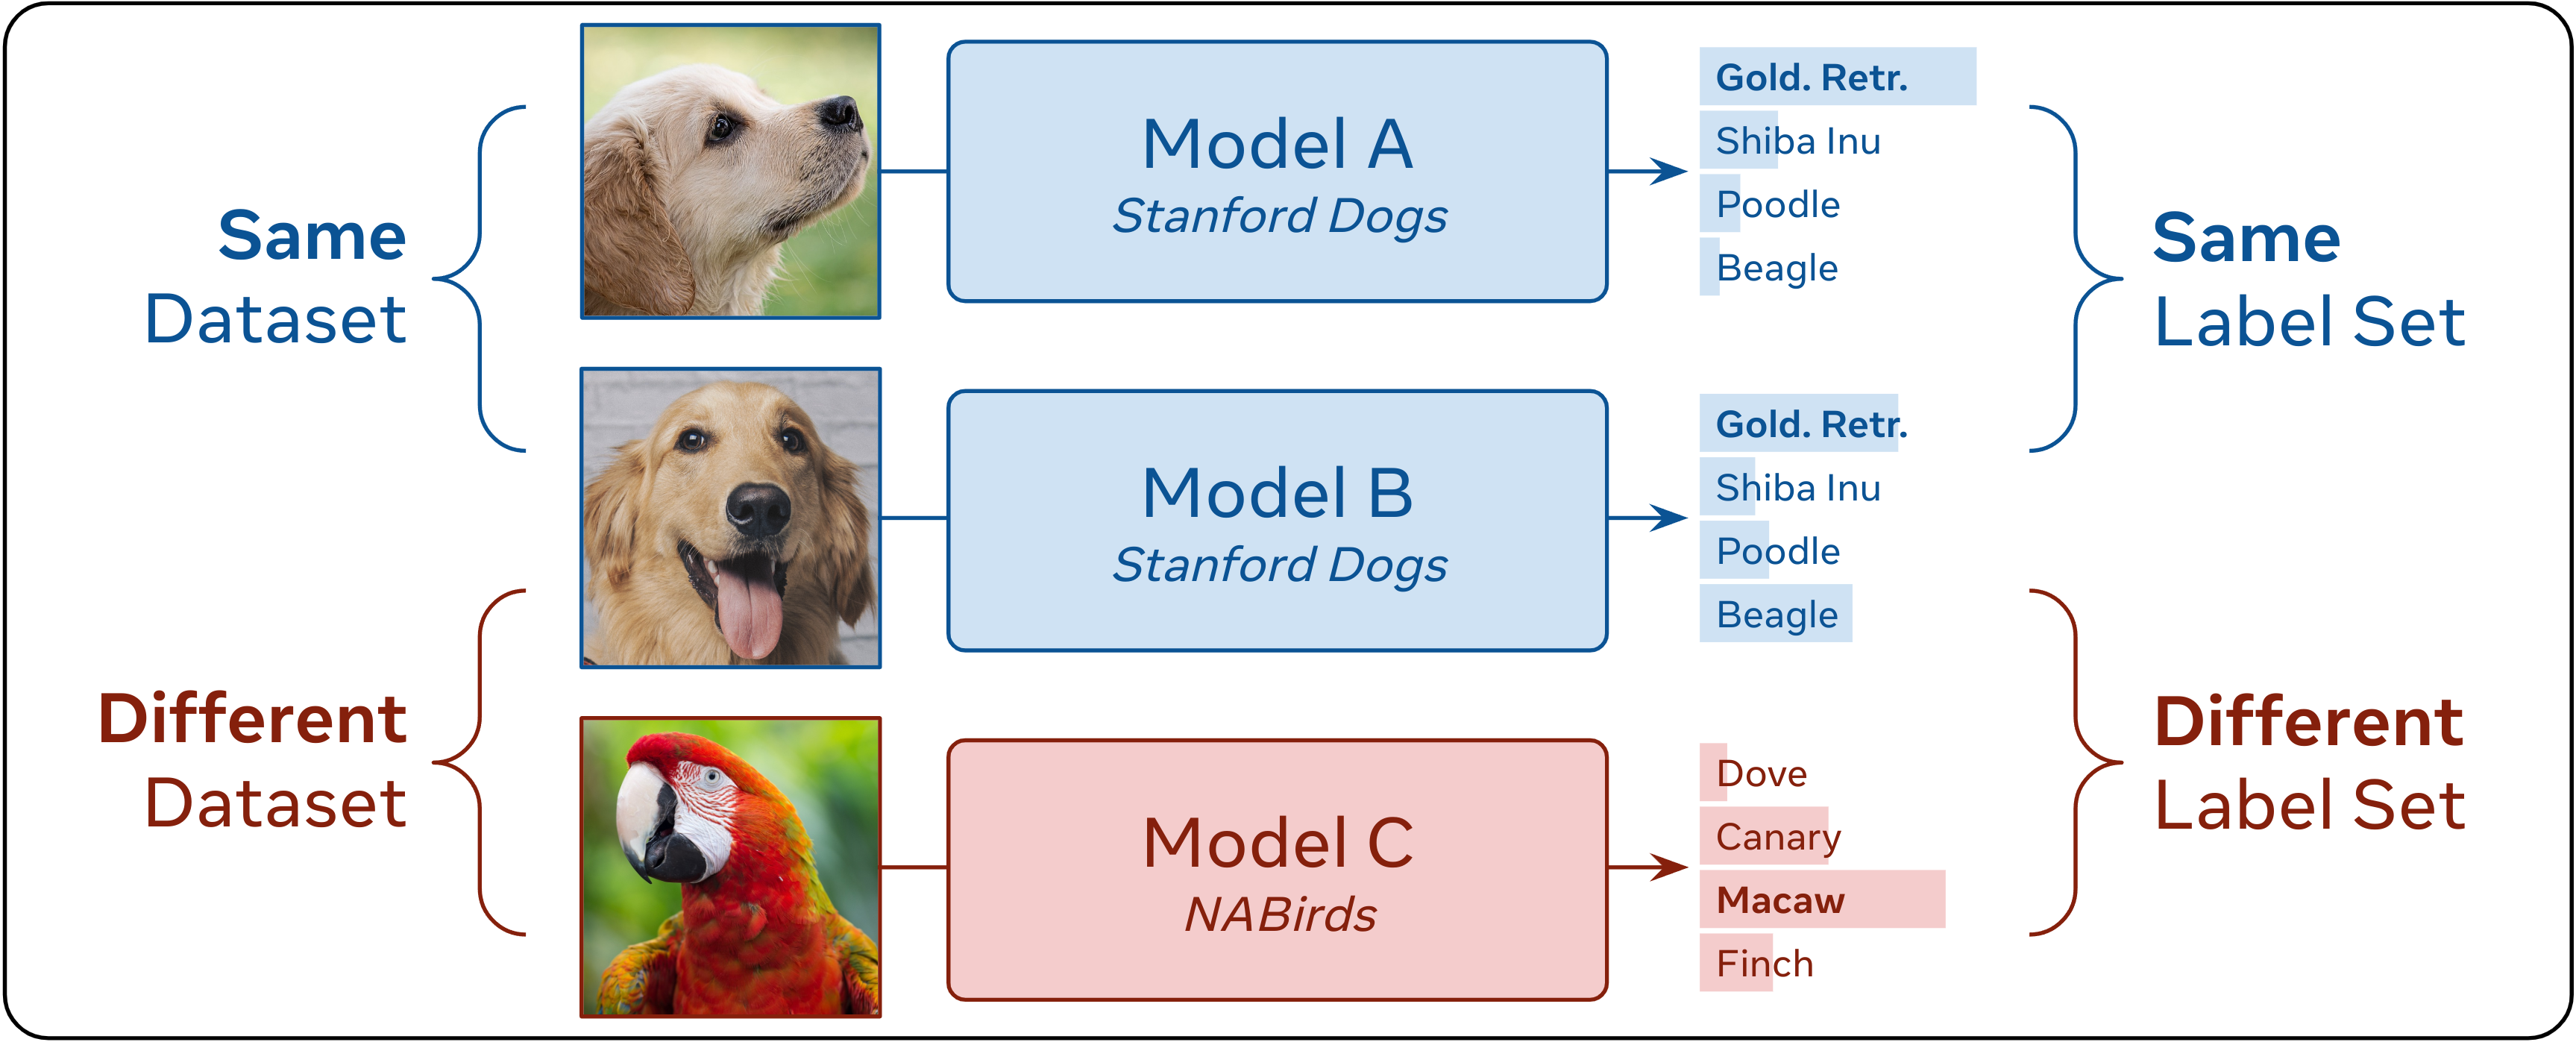
\includegraphics[width=\linewidth]{figures/imgs/vs_prior_work.png}
%     \caption{{\bf Our Setting.} Prior work \cite{wortsman2022model,ainsworth2022git,jordan2022repair}
%     focuses on merging models from the \modelb{\textbf{same} dataset} with the \modelb{\textbf{same} label sets}: e.g., merging two models both trained to classify dog breeds. In this work, we remove that restriction and ``zip'' models that can come from \modela{\textbf{different} datasets} and have \modela{\textbf{different} label sets}: e.g., merging a model that classifies dog breeds with one that classifies bird species.
%     }
%     \label{fig:capabilities}
%     % \includegraphics[width=\linewidth]{figures/imgs/random_r_experiment.png}
    
%     % \captionof{figure}{\textbf{Token Merging Schedule.} Our default constant merging schedule is close to optimal when compared to 15k randomly sampled merging schedules on an AugReg ViT-B/16. }
%     % \label{fig:r_ablation}
% }\end{minipage}
% \end{figure}




\begin{figure}[t]
\centering
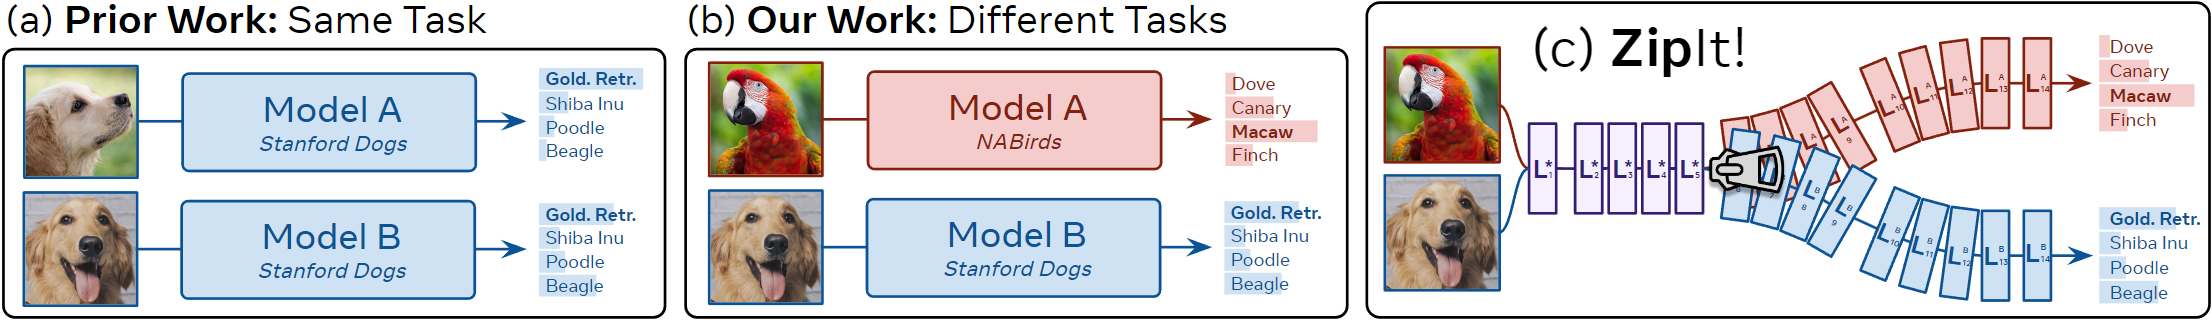
\includegraphics[width=\linewidth]{figures/imgs/concept_and_capabilities.png}
    \caption{
    {\bf Setting and \name{}} (a) Prior work merges differently initialized models from the \modelb{\textbf{same} dataset} with the \modelb{\textbf{same} label sets}: e.g., merging two models both trained to classify dog breeds. (b) Our setting expands this to merging models from \modela{\textbf{different} datasets} with \modela{\textbf{different} label sets}: e.g., merging a model that classifies dog breeds with one that classifies bird species. (c) {\bf \name{}}\ merges these models \textit{without retraining} by identifying shared features.
    }
    \label{fig:concept_and_capabilities}
\end{figure}




% However, while these deep models are extremely powerful, they suffer from a potentially debilitating issue: they can only perform the task they were trained on. If we want to expand an existing model's capabilities, we run into many potential issues. If we try training the model on an additional task, we face catastrophic forgetting \cite{kirkpatrick2017overcoming,li2017learning,de2021continual}. If we evaluate the same model on different data without adaptation, we often find it doesn't generalize to out of domain samples \cite{blanchard2011generalizing,muandet2013domain,wang2022generalizing}. We can try so called ``intervention'' strategies \cite{wang2022generalizing,de2021continual} to mitigate these effects, but these often require further training which can be expensive.
% 


% \begin{figure}[b]
% \centering

% \begin{minipage}{0.48\linewidth}{
%     % \centering
%     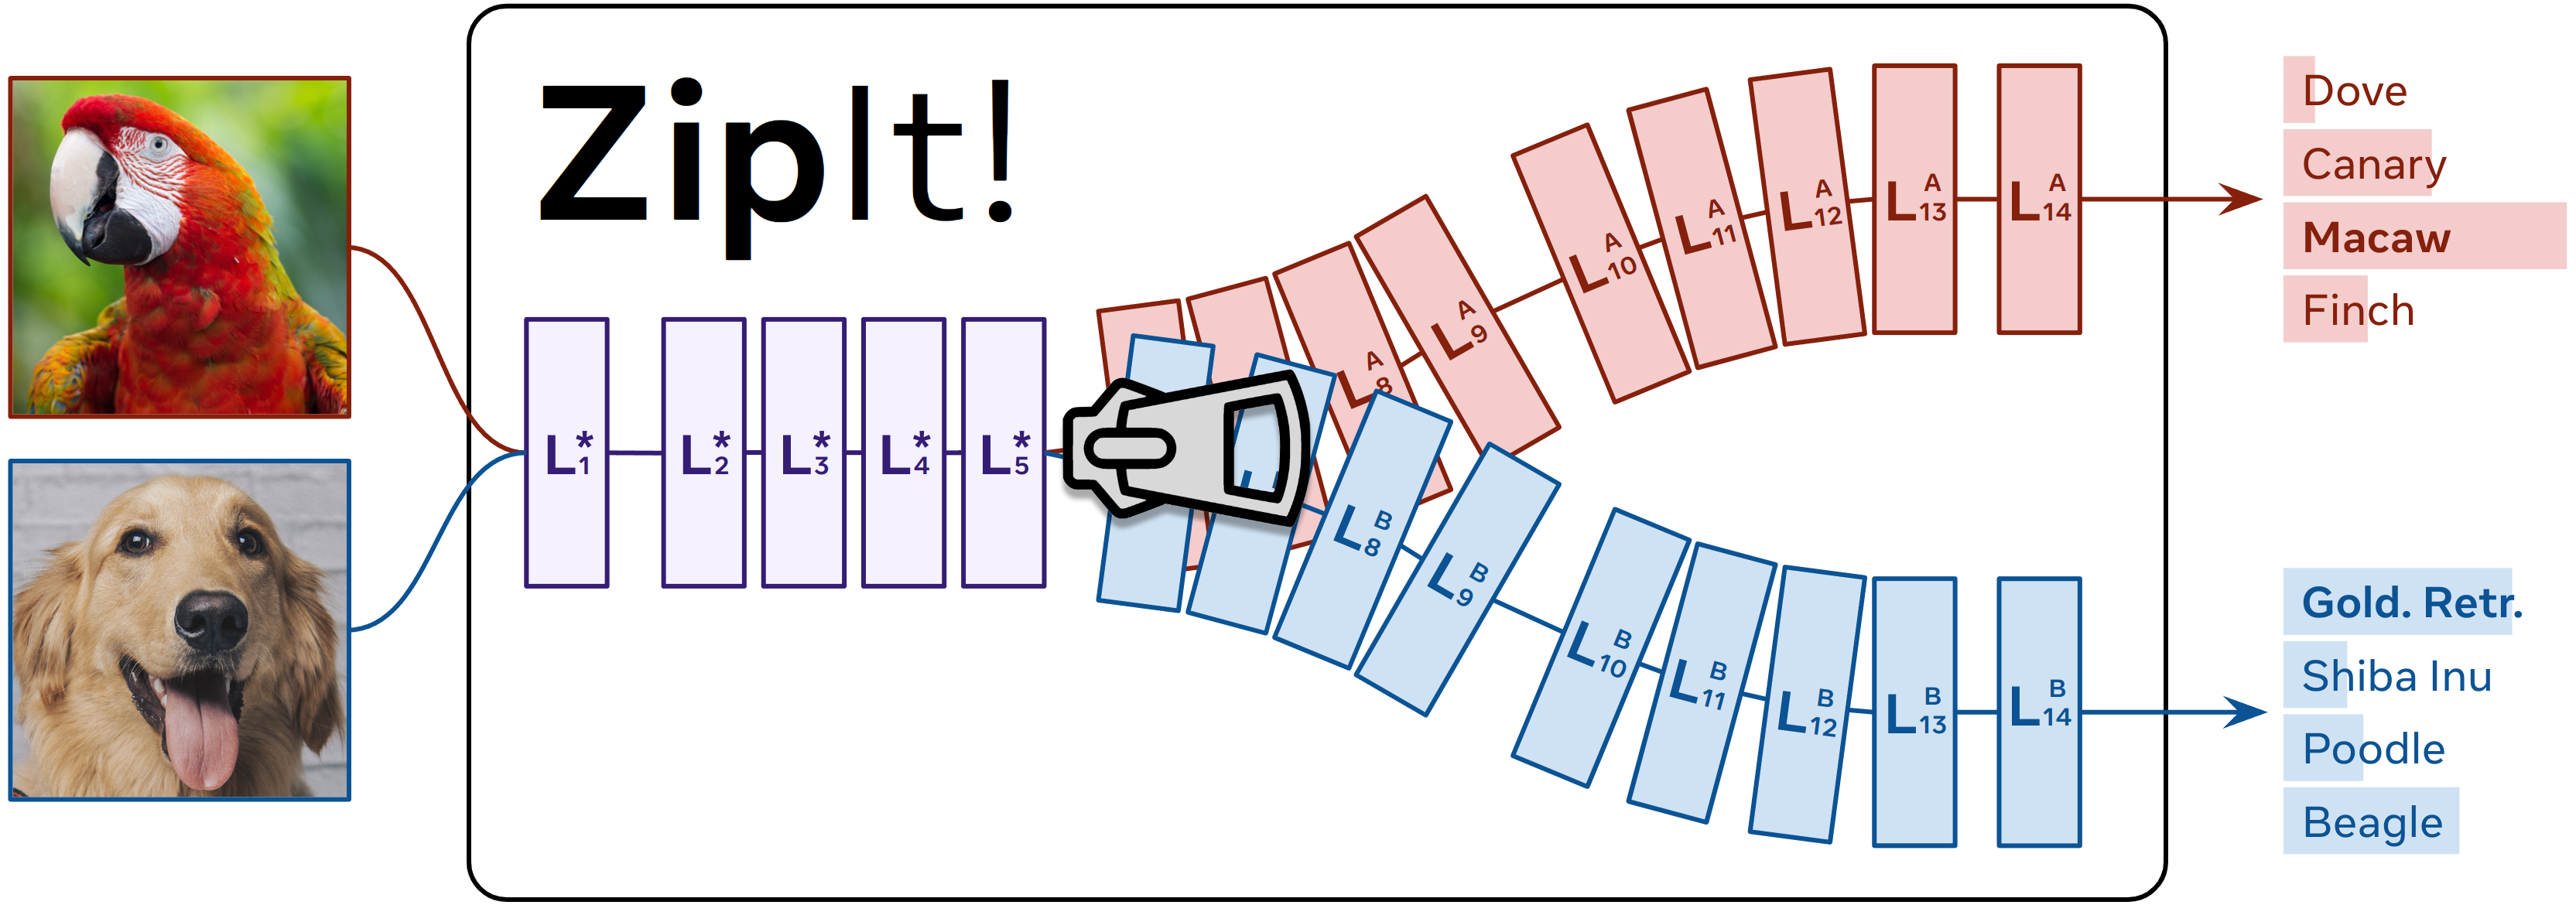
\includegraphics[width=\linewidth]{figures/imgs/concept.png}
%     \caption{{\bf \name{}} merges models trained on completely separate tasks \textit{without any additional training} by identifying their shared features.
%     Depending on the architecture and task, \name{} can nearly match their ensemble performance.
%     }
%     \label{fig:concept}
% }\end{minipage}
% \hspace{1em}
% \begin{minipage}{0.48\linewidth}{
%     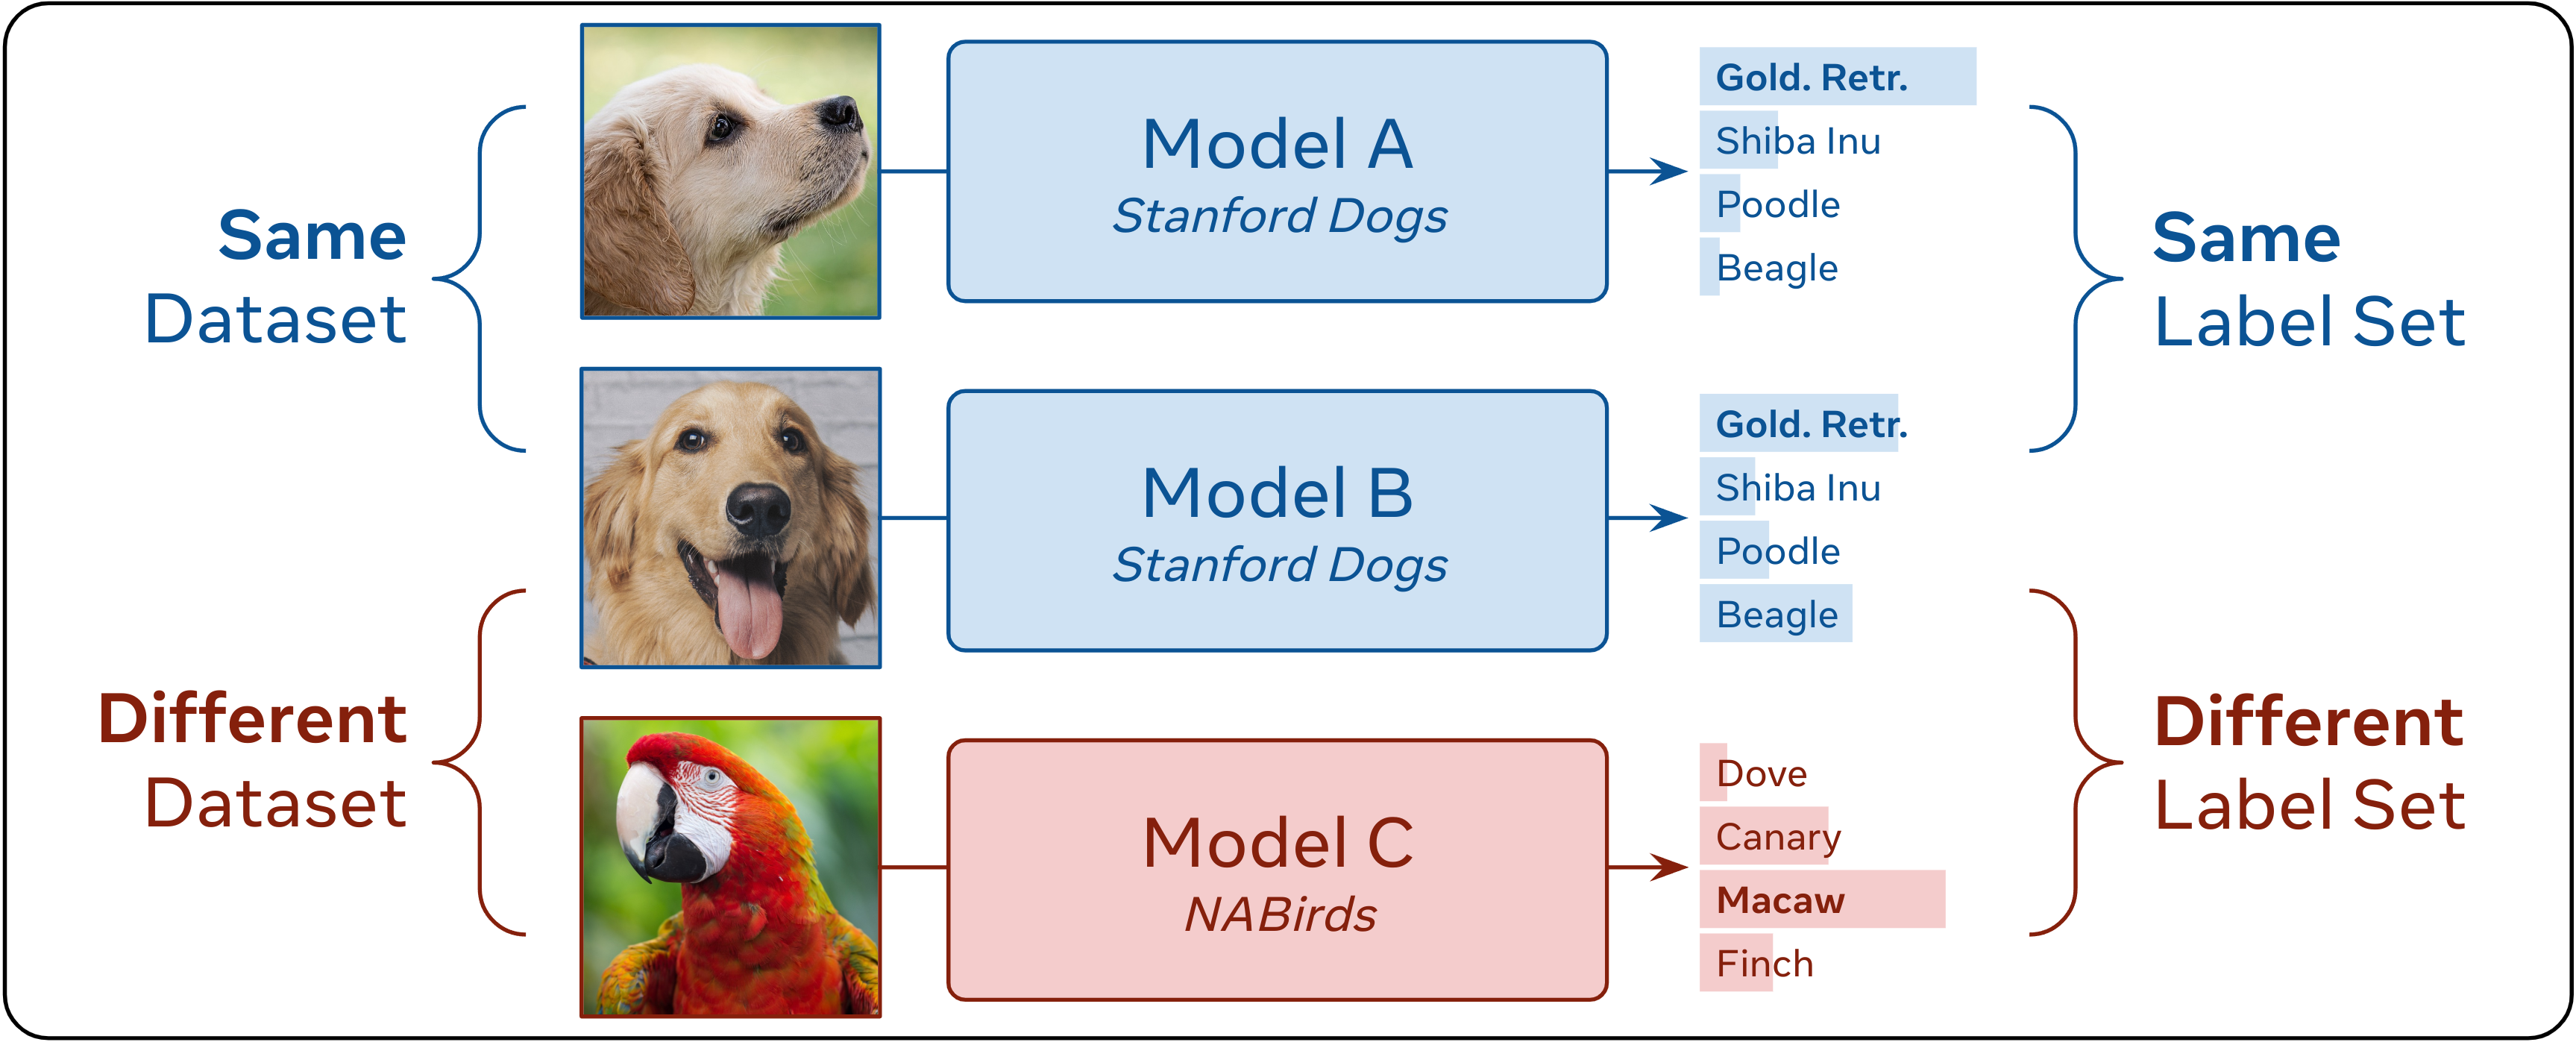
\includegraphics[width=\linewidth]{figures/imgs/vs_prior_work.png}
%     \caption{{\bf Our Setting.} Prior work \cite{wortsman2022model,ainsworth2022git,jordan2022repair}
%     focuses on merging models from the \modelb{\textbf{same} dataset} with the \modelb{\textbf{same} label sets}: e.g., merging two models both trained to classify dog breeds. In this work, we remove that restriction and ``zip'' models that can come from \modela{\textbf{different} datasets} and have \modela{\textbf{different} label sets}: e.g., merging a model that classifies dog breeds with one that classifies bird species.
%     }
%     \label{fig:capabilities}
%     % \includegraphics[width=\linewidth]{figures/imgs/random_r_experiment.png}
    
%     % \captionof{figure}{\textbf{Token Merging Schedule.} Our default constant merging schedule is close to optimal when compared to 15k randomly sampled merging schedules on an AugReg ViT-B/16. }
%     % \label{fig:r_ablation}
% }\end{minipage}
% \end{figure}




\begin{figure}[t]
\centering
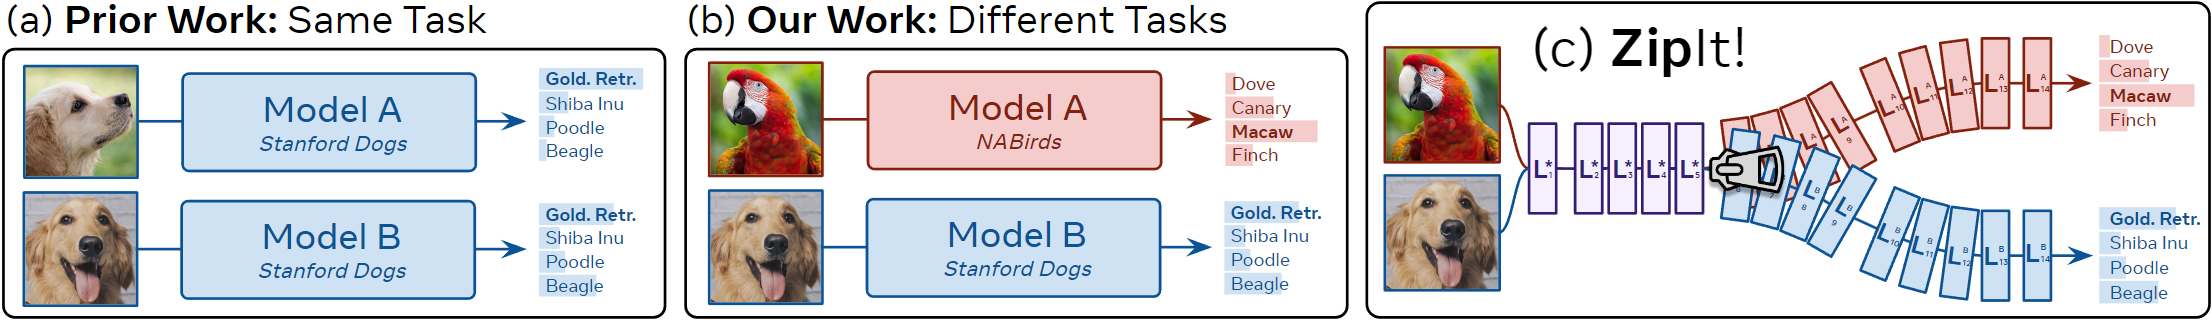
\includegraphics[width=\linewidth]{figures/imgs/concept_and_capabilities.png}
    \caption{
    {\bf Setting and \name{}} (a) Prior work merges differently initialized models from the \modelb{\textbf{same} dataset} with the \modelb{\textbf{same} label sets}: e.g., merging two models both trained to classify dog breeds. (b) Our setting expands this to merging models from \modela{\textbf{different} datasets} with \modela{\textbf{different} label sets}: e.g., merging a model that classifies dog breeds with one that classifies bird species. (c) {\bf \name{}}\ merges these models \textit{without retraining} by identifying shared features.
    }
    \label{fig:concept_and_capabilities}
\end{figure}


% There are
% %,  of course, 
% a plethora of existing, carefully tuned models out there for many tasks. But despite these models often sharing the same core architectural backbone (e.g., ResNet-50~\cite{he2015deep}), no method yet exists that can easily combine models trained on disjoint tasks. We're either stuck ensembling them, which requires evaluating each model individually, or jointly training a new model through distillation~\cite{li2020knowledge}. Both can be prohibitively expensive with the modern trend of ever increasing architecture and dataset scales \cite{dosovitskiy2020image,zhai2022scaling,dehghani2023scalingvit22b}.
% Instead, it would be nice if we could simply ``zip'' these models together so that any redundant features between them only need to be computed once, \textit{without} any additional training.

% Recently, the idea of combining multiple models into one has started to gain traction in the vision community. 
Combining multiple models into one has recently started to gain traction in the vision community.
Model Soups \cite{wortsman2022model} can add multiple models finetuned from the same pretrained initialization to improve accuracy and robustness. Git Re-Basin \cite{ainsworth2022git} generalizes further to models trained on the same data but with different initializations, though with a significant accuracy drop. REPAIR \cite{jordan2022repair} improves on Git Re-Basin by adding new parameters and adjusting model batch norms where applicable.
However, all of these methods only combine models trained on the same task.
In this paper, we take this line of work to a logical extreme: merging differently initialized models trained on \textit{completely separate} tasks (see Fig.~\ref{fig:concept_and_capabilities}\hyperref[fig:concept_and_capabilities]{ab}).
% While 
We show
that this is an incredibly difficult problem for prior work 
% we 
and
employ two simple strategies to make it feasible.

First, we note that prior work focuses on \textit{permuting} one model to the other when merging them. This creates a 1-1 mapping between the two models, inherently assuming that most features \textit{across} them are correlated. Since this isn't necessarily the case for models trained on different tasks, we cannot rely on permutation alone. 
Instead, we generalize model merging to support ``zipping'' any combination of correlated features \textit{within} and \textit{across} each model.
% Instead, we exploit redundancy \textit{within} each model as well. 
% To do this, we generalize model merging to support ``zipping'' any combination of features \textit{within} and \textit{across} each model.
We find that on some tasks, this alone improves accuracy \textbf{by up to 20\%} vs. 
permutation-based approaches.
% Git Re-basin \cite{ainsworth2022git} applied in this setting and an even stronger permutation baseline that we implement.
Moreover, we prove that merging within models can yield a better result in the theoretical setting of \citet{entezari2021role}.

Second, existing methods merge \textit{the entire network}. While this might work for extremely similar models trained in the same setting, the features of models trained on disjoint tasks become less correlated over the course of the network \cite{kornblith2019similarity}. To solve this, we introduce \textit{partial zipping}, where we only ``zip'' up to a specified layer. Afterward, we feed the merged model's outputs to the remaining unmerged layers of the original networks, creating a multi-head model. Depending on task difficulty, this can improve accuracy \textbf{by over 15\%} while still keeping most layers merged.


Incorporating both of these strategies, we introduce \name{}\ (Fig.~\ref{fig:concept_and_capabilities}\hyperref[fig:concept_and_capabilities]{c}), a general method for ``zipping'' any number of models trained on different tasks into a single multitask model \textit{without retraining}.
By deriving a general graph-based algorithm for merging and unmerging (Sec.~\ref{sec:approach}), we can zip models of the same architecture together, 
merge features \textit{within} each model,
and partially zip them to create a multi-task model.
We validate our approach by merging models trained on entirely disjoint sets of CIFAR \cite{krizhevsky2009cifar} and ImageNet \cite{deng2009imagenet} categories, as well as merging several models trained on completely independent datasets into one, significantly outperforming prior work (Sec.~\ref{sec:results}). 
Finally, we ablate and analyze our method's capabilities on these scenarios (Sec.~\ref{sec:ablations}).